% =====================================================================
%  DORI signal chain, for the METHODS column of the poster.
%
%  Deliberately between the two extremes: it names every stage the reader
%  needs, with a sketch of what the signal looks like as it goes, but it is
%  not a schematic. No component values, no op-amps, no wires.
%
%  Self-contained TikZ. Needs only \usepackage{tikz} plus the two libraries
%  below, which your poster already loads. Use it with
%      \resizebox{\linewidth}{!}{% =====================================================================
%  DORI signal chain, for the METHODS column of the poster.
%
%  Deliberately between the two extremes: it names every stage the reader
%  needs, with a sketch of what the signal looks like as it goes, but it is
%  not a schematic. No component values, no op-amps, no wires.
%
%  Self-contained TikZ. Needs only \usepackage{tikz} plus the two libraries
%  below, which your poster already loads. Use it with
%      \resizebox{\linewidth}{!}{% =====================================================================
%  DORI signal chain, for the METHODS column of the poster.
%
%  Deliberately between the two extremes: it names every stage the reader
%  needs, with a sketch of what the signal looks like as it goes, but it is
%  not a schematic. No component values, no op-amps, no wires.
%
%  Self-contained TikZ. Needs only \usepackage{tikz} plus the two libraries
%  below, which your poster already loads. Use it with
%      \resizebox{\linewidth}{!}{% =====================================================================
%  DORI signal chain, for the METHODS column of the poster.
%
%  Deliberately between the two extremes: it names every stage the reader
%  needs, with a sketch of what the signal looks like as it goes, but it is
%  not a schematic. No component values, no op-amps, no wires.
%
%  Self-contained TikZ. Needs only \usepackage{tikz} plus the two libraries
%  below, which your poster already loads. Use it with
%      \resizebox{\linewidth}{!}{\input{methods_figure.tex}}
%
%  The picture is drawn about 20 cm wide and 9.5 cm tall, so in a 24.6 cm
%  column it prints roughly 24.6 x 11.7 cm and the box titles come out near
%  23 pt. Everything is positioned from the numbers in the two rows below.
% =====================================================================

\usetikzlibrary{arrows.meta,positioning,decorations.pathmorphing}

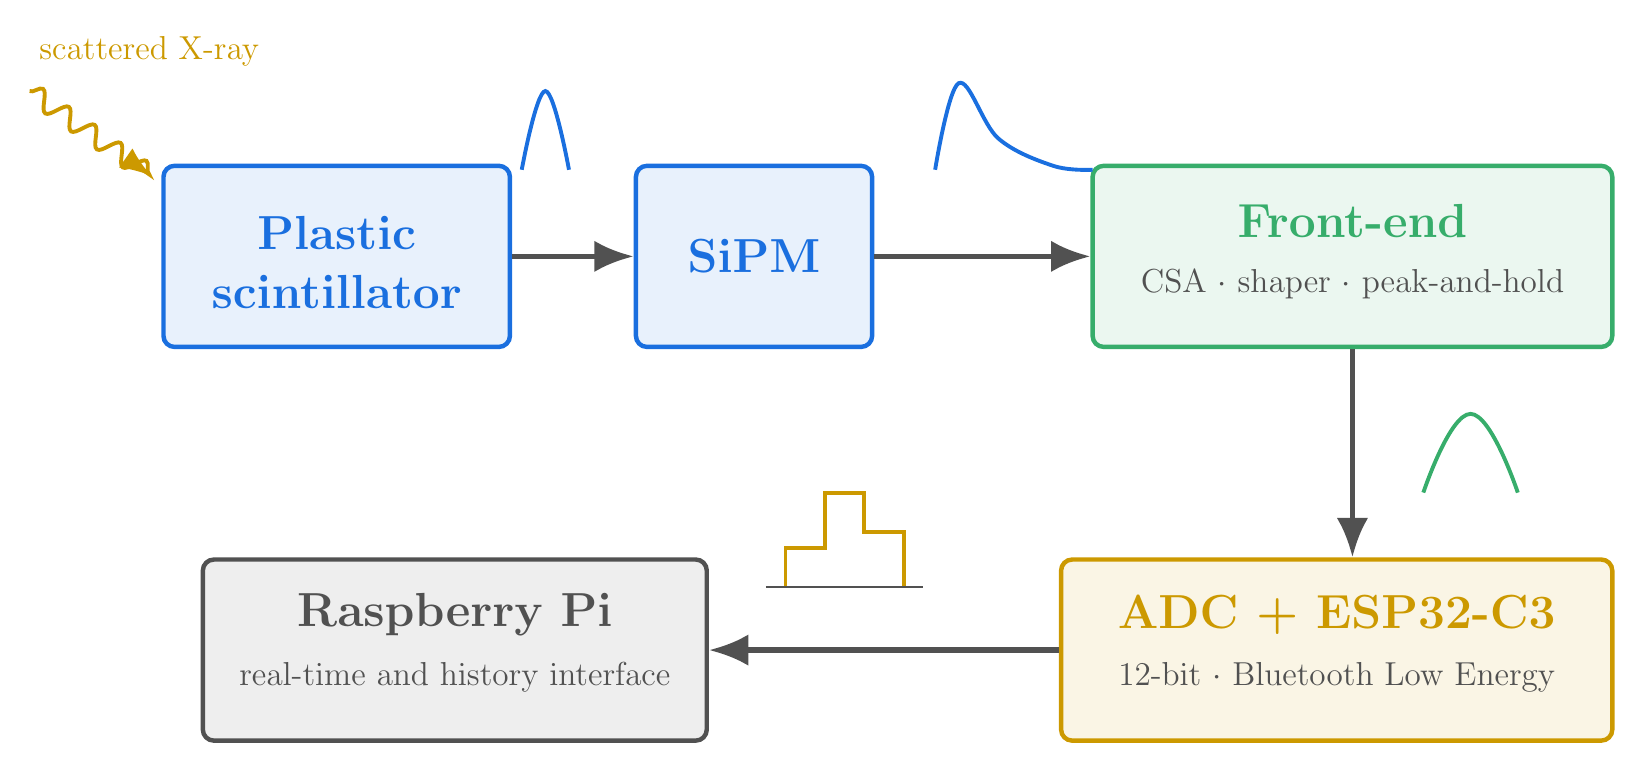
\begin{tikzpicture}[x=1cm, y=1cm,
  % ---- colours: your palette -----------------------------------------
  /utils/exec={%
    \definecolor{figblue}  {RGB}{ 26,111,223}%
    \definecolor{figgreen} {RGB}{ 55,173,107}%
    \definecolor{figyellow}{RGB}{204,153,  0}%
    \definecolor{figgrey}  {RGB}{ 81, 81, 81}%
  },
  % ---- one style per box, change fill/draw here ------------------------
  blk/.style={
    rounded corners=4pt, draw=#1, line width=1.6pt, fill=#1!10,
    align=center, inner sep=6pt, text=#1
  },
  ttl/.style={font=\LARGE\bfseries},
  sub/.style={font=\large, text=figgrey},
  flow/.style={draw=figgrey, line width=2pt, -{Latex[length=5mm,width=4mm]}},
  wave/.style={draw=#1, line width=1.4pt},
]

% =====================================================================
%  ROW 1 : detection and analogue front end
% =====================================================================
\node[blk=figblue,  minimum width=4.4cm, minimum height=2.3cm] (scint) at (2.7,6.4) {};
\node[ttl, text=figblue] at (2.7,6.7) {Plastic};
\node[ttl, text=figblue] at (2.7,5.95) {scintillator};

\node[blk=figblue,  minimum width=3.0cm, minimum height=2.3cm] (sipm)  at (8.0,6.4) {};
\node[ttl, text=figblue] at (8.0,6.4) {SiPM};

\node[blk=figgreen, minimum width=6.6cm, minimum height=2.3cm] (fe)    at (15.6,6.4) {};
\node[ttl, text=figgreen] at (15.6,6.85) {Front-end};
\node[sub]                at (15.6,6.05) {CSA $\cdot$ shaper $\cdot$ peak-and-hold};

% =====================================================================
%  ROW 2 : digitisation and readout
% =====================================================================
\node[blk=figyellow, minimum width=7.0cm, minimum height=2.3cm] (adc) at (15.4,1.4) {};
\node[ttl, text=figyellow] at (15.4,1.85) {ADC + ESP32-C3};
\node[sub]                 at (15.4,1.05) {12-bit $\cdot$ Bluetooth Low Energy};

\node[blk=figgrey, minimum width=6.4cm, minimum height=2.3cm] (rpi) at (4.2,1.4) {};
\node[ttl, text=figgrey] at (4.2,1.85) {Raspberry Pi};
\node[sub]               at (4.2,1.05) {real-time and history interface};

% =====================================================================
%  FLOW
% =====================================================================
\draw[flow] (scint) -- (sipm);
\draw[flow] (sipm)  -- (fe);
\draw[flow] (fe.south) -- (fe.south |- adc.north);
\draw[flow] (adc) -- (rpi);

% incoming scattered X-ray
\draw[wave=figyellow, decorate, decoration={snake, amplitude=1.2mm, segment length=4mm},
      -{Latex[length=4mm,width=3mm]}] (-1.2,8.5) -- (0.35,7.42);
\node[font=\large, text=figyellow, anchor=west] at (-1.2,9.0) {scattered X-ray};

% =====================================================================
%  WHAT THE SIGNAL LOOKS LIKE, one sketch per hand-off
% =====================================================================
% light flash out of the scintillator
\draw[wave=figblue] plot[smooth,tension=0.7] coordinates
      {(5.05,7.5) (5.35,8.5) (5.65,7.5)};
% raw SiPM pulse: fast rise, long tail
\draw[wave=figblue] plot[smooth,tension=0.6] coordinates
      {(10.3,7.5) (10.6,8.6) (11.1,7.9) (11.8,7.55) (12.3,7.5)};
% shaped pulse, beside the vertical arrow
\draw[wave=figgreen] plot[smooth,tension=0.8] coordinates
      {(16.5,3.4) (17.1,4.4) (17.7,3.4)};
% digitised spectrum, above the arrow back to the interface
\draw[wave=figyellow] (8.4,2.2) -- (8.4,2.7) -- (8.9,2.7) -- (8.9,3.4)
                   -- (9.4,3.4) -- (9.4,2.9) -- (9.9,2.9) -- (9.9,2.2);
\draw[figgrey, line width=1pt] (8.15,2.2) -- (10.15,2.2);

\end{tikzpicture}
}
%
%  The picture is drawn about 20 cm wide and 9.5 cm tall, so in a 24.6 cm
%  column it prints roughly 24.6 x 11.7 cm and the box titles come out near
%  23 pt. Everything is positioned from the numbers in the two rows below.
% =====================================================================

\usetikzlibrary{arrows.meta,positioning,decorations.pathmorphing}

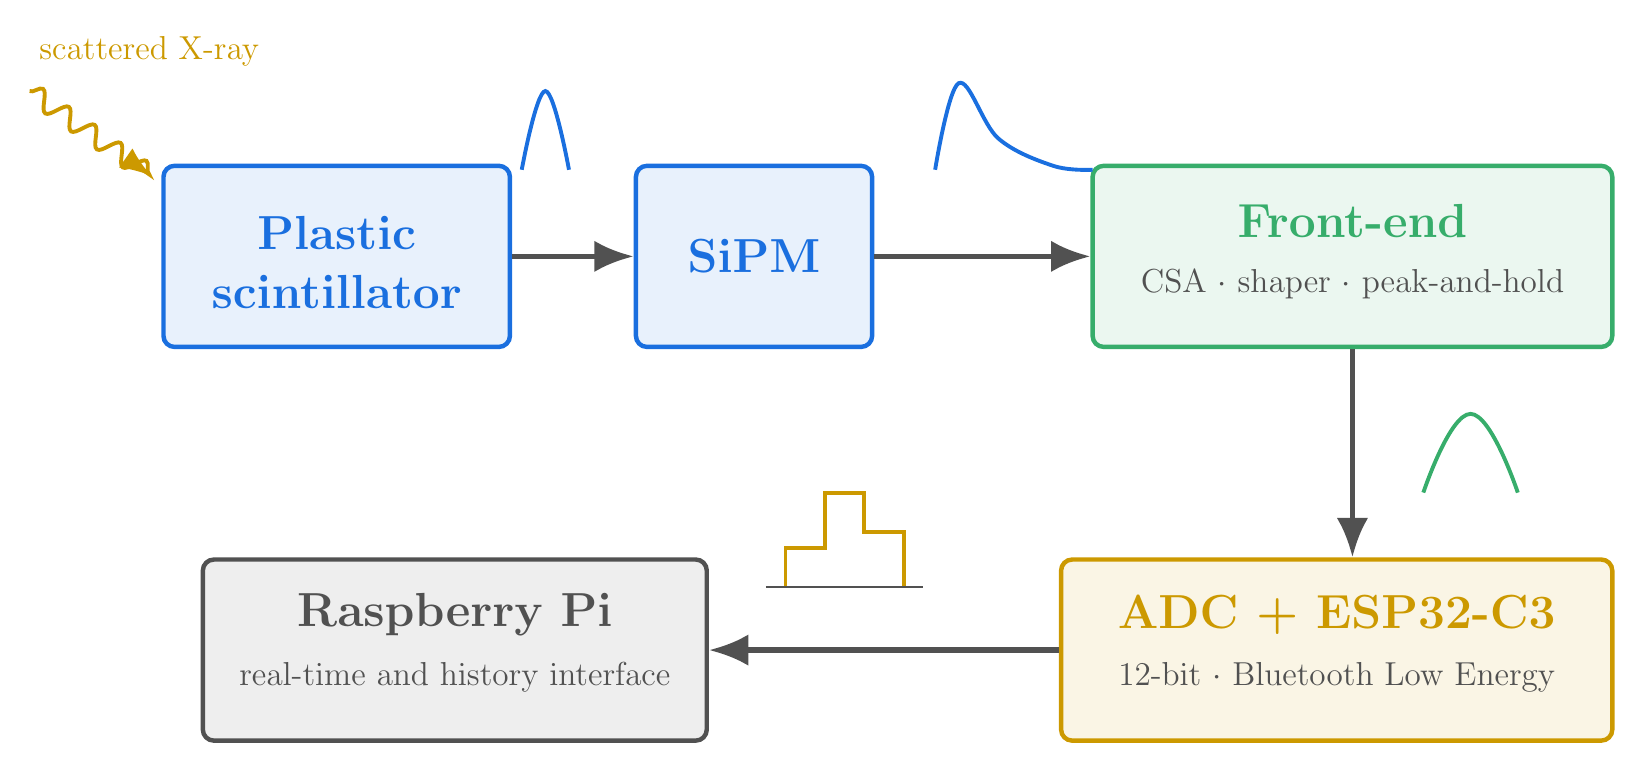
\begin{tikzpicture}[x=1cm, y=1cm,
  % ---- colours: your palette -----------------------------------------
  /utils/exec={%
    \definecolor{figblue}  {RGB}{ 26,111,223}%
    \definecolor{figgreen} {RGB}{ 55,173,107}%
    \definecolor{figyellow}{RGB}{204,153,  0}%
    \definecolor{figgrey}  {RGB}{ 81, 81, 81}%
  },
  % ---- one style per box, change fill/draw here ------------------------
  blk/.style={
    rounded corners=4pt, draw=#1, line width=1.6pt, fill=#1!10,
    align=center, inner sep=6pt, text=#1
  },
  ttl/.style={font=\LARGE\bfseries},
  sub/.style={font=\large, text=figgrey},
  flow/.style={draw=figgrey, line width=2pt, -{Latex[length=5mm,width=4mm]}},
  wave/.style={draw=#1, line width=1.4pt},
]

% =====================================================================
%  ROW 1 : detection and analogue front end
% =====================================================================
\node[blk=figblue,  minimum width=4.4cm, minimum height=2.3cm] (scint) at (2.7,6.4) {};
\node[ttl, text=figblue] at (2.7,6.7) {Plastic};
\node[ttl, text=figblue] at (2.7,5.95) {scintillator};

\node[blk=figblue,  minimum width=3.0cm, minimum height=2.3cm] (sipm)  at (8.0,6.4) {};
\node[ttl, text=figblue] at (8.0,6.4) {SiPM};

\node[blk=figgreen, minimum width=6.6cm, minimum height=2.3cm] (fe)    at (15.6,6.4) {};
\node[ttl, text=figgreen] at (15.6,6.85) {Front-end};
\node[sub]                at (15.6,6.05) {CSA $\cdot$ shaper $\cdot$ peak-and-hold};

% =====================================================================
%  ROW 2 : digitisation and readout
% =====================================================================
\node[blk=figyellow, minimum width=7.0cm, minimum height=2.3cm] (adc) at (15.4,1.4) {};
\node[ttl, text=figyellow] at (15.4,1.85) {ADC + ESP32-C3};
\node[sub]                 at (15.4,1.05) {12-bit $\cdot$ Bluetooth Low Energy};

\node[blk=figgrey, minimum width=6.4cm, minimum height=2.3cm] (rpi) at (4.2,1.4) {};
\node[ttl, text=figgrey] at (4.2,1.85) {Raspberry Pi};
\node[sub]               at (4.2,1.05) {real-time and history interface};

% =====================================================================
%  FLOW
% =====================================================================
\draw[flow] (scint) -- (sipm);
\draw[flow] (sipm)  -- (fe);
\draw[flow] (fe.south) -- (fe.south |- adc.north);
\draw[flow] (adc) -- (rpi);

% incoming scattered X-ray
\draw[wave=figyellow, decorate, decoration={snake, amplitude=1.2mm, segment length=4mm},
      -{Latex[length=4mm,width=3mm]}] (-1.2,8.5) -- (0.35,7.42);
\node[font=\large, text=figyellow, anchor=west] at (-1.2,9.0) {scattered X-ray};

% =====================================================================
%  WHAT THE SIGNAL LOOKS LIKE, one sketch per hand-off
% =====================================================================
% light flash out of the scintillator
\draw[wave=figblue] plot[smooth,tension=0.7] coordinates
      {(5.05,7.5) (5.35,8.5) (5.65,7.5)};
% raw SiPM pulse: fast rise, long tail
\draw[wave=figblue] plot[smooth,tension=0.6] coordinates
      {(10.3,7.5) (10.6,8.6) (11.1,7.9) (11.8,7.55) (12.3,7.5)};
% shaped pulse, beside the vertical arrow
\draw[wave=figgreen] plot[smooth,tension=0.8] coordinates
      {(16.5,3.4) (17.1,4.4) (17.7,3.4)};
% digitised spectrum, above the arrow back to the interface
\draw[wave=figyellow] (8.4,2.2) -- (8.4,2.7) -- (8.9,2.7) -- (8.9,3.4)
                   -- (9.4,3.4) -- (9.4,2.9) -- (9.9,2.9) -- (9.9,2.2);
\draw[figgrey, line width=1pt] (8.15,2.2) -- (10.15,2.2);

\end{tikzpicture}
}
%
%  The picture is drawn about 20 cm wide and 9.5 cm tall, so in a 24.6 cm
%  column it prints roughly 24.6 x 11.7 cm and the box titles come out near
%  23 pt. Everything is positioned from the numbers in the two rows below.
% =====================================================================

\usetikzlibrary{arrows.meta,positioning,decorations.pathmorphing}

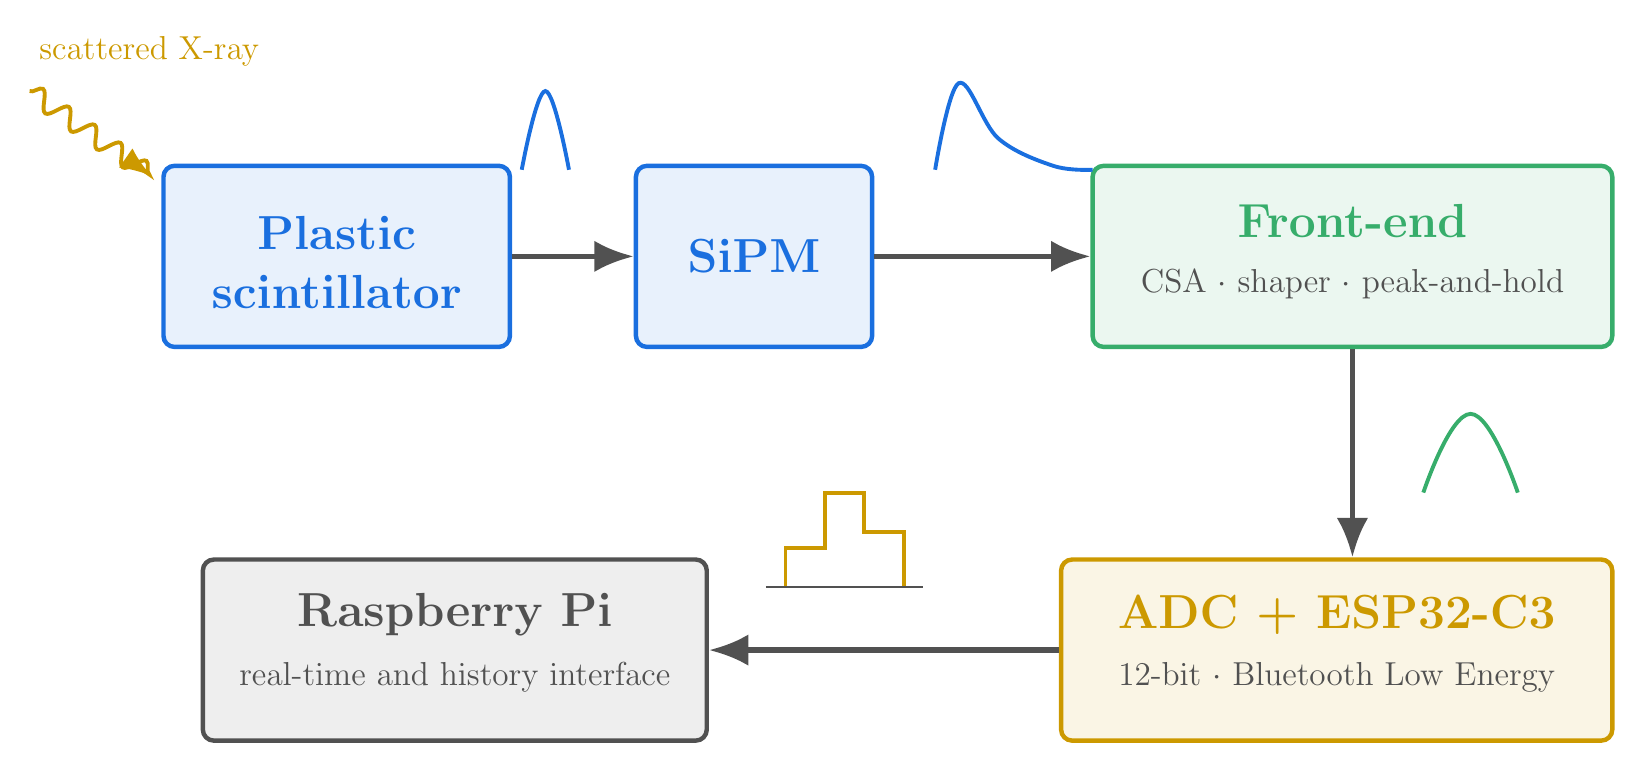
\begin{tikzpicture}[x=1cm, y=1cm,
  % ---- colours: your palette -----------------------------------------
  /utils/exec={%
    \definecolor{figblue}  {RGB}{ 26,111,223}%
    \definecolor{figgreen} {RGB}{ 55,173,107}%
    \definecolor{figyellow}{RGB}{204,153,  0}%
    \definecolor{figgrey}  {RGB}{ 81, 81, 81}%
  },
  % ---- one style per box, change fill/draw here ------------------------
  blk/.style={
    rounded corners=4pt, draw=#1, line width=1.6pt, fill=#1!10,
    align=center, inner sep=6pt, text=#1
  },
  ttl/.style={font=\LARGE\bfseries},
  sub/.style={font=\large, text=figgrey},
  flow/.style={draw=figgrey, line width=2pt, -{Latex[length=5mm,width=4mm]}},
  wave/.style={draw=#1, line width=1.4pt},
]

% =====================================================================
%  ROW 1 : detection and analogue front end
% =====================================================================
\node[blk=figblue,  minimum width=4.4cm, minimum height=2.3cm] (scint) at (2.7,6.4) {};
\node[ttl, text=figblue] at (2.7,6.7) {Plastic};
\node[ttl, text=figblue] at (2.7,5.95) {scintillator};

\node[blk=figblue,  minimum width=3.0cm, minimum height=2.3cm] (sipm)  at (8.0,6.4) {};
\node[ttl, text=figblue] at (8.0,6.4) {SiPM};

\node[blk=figgreen, minimum width=6.6cm, minimum height=2.3cm] (fe)    at (15.6,6.4) {};
\node[ttl, text=figgreen] at (15.6,6.85) {Front-end};
\node[sub]                at (15.6,6.05) {CSA $\cdot$ shaper $\cdot$ peak-and-hold};

% =====================================================================
%  ROW 2 : digitisation and readout
% =====================================================================
\node[blk=figyellow, minimum width=7.0cm, minimum height=2.3cm] (adc) at (15.4,1.4) {};
\node[ttl, text=figyellow] at (15.4,1.85) {ADC + ESP32-C3};
\node[sub]                 at (15.4,1.05) {12-bit $\cdot$ Bluetooth Low Energy};

\node[blk=figgrey, minimum width=6.4cm, minimum height=2.3cm] (rpi) at (4.2,1.4) {};
\node[ttl, text=figgrey] at (4.2,1.85) {Raspberry Pi};
\node[sub]               at (4.2,1.05) {real-time and history interface};

% =====================================================================
%  FLOW
% =====================================================================
\draw[flow] (scint) -- (sipm);
\draw[flow] (sipm)  -- (fe);
\draw[flow] (fe.south) -- (fe.south |- adc.north);
\draw[flow] (adc) -- (rpi);

% incoming scattered X-ray
\draw[wave=figyellow, decorate, decoration={snake, amplitude=1.2mm, segment length=4mm},
      -{Latex[length=4mm,width=3mm]}] (-1.2,8.5) -- (0.35,7.42);
\node[font=\large, text=figyellow, anchor=west] at (-1.2,9.0) {scattered X-ray};

% =====================================================================
%  WHAT THE SIGNAL LOOKS LIKE, one sketch per hand-off
% =====================================================================
% light flash out of the scintillator
\draw[wave=figblue] plot[smooth,tension=0.7] coordinates
      {(5.05,7.5) (5.35,8.5) (5.65,7.5)};
% raw SiPM pulse: fast rise, long tail
\draw[wave=figblue] plot[smooth,tension=0.6] coordinates
      {(10.3,7.5) (10.6,8.6) (11.1,7.9) (11.8,7.55) (12.3,7.5)};
% shaped pulse, beside the vertical arrow
\draw[wave=figgreen] plot[smooth,tension=0.8] coordinates
      {(16.5,3.4) (17.1,4.4) (17.7,3.4)};
% digitised spectrum, above the arrow back to the interface
\draw[wave=figyellow] (8.4,2.2) -- (8.4,2.7) -- (8.9,2.7) -- (8.9,3.4)
                   -- (9.4,3.4) -- (9.4,2.9) -- (9.9,2.9) -- (9.9,2.2);
\draw[figgrey, line width=1pt] (8.15,2.2) -- (10.15,2.2);

\end{tikzpicture}
}
%
%  The picture is drawn about 20 cm wide and 9.5 cm tall, so in a 24.6 cm
%  column it prints roughly 24.6 x 11.7 cm and the box titles come out near
%  23 pt. Everything is positioned from the numbers in the two rows below.
% =====================================================================

\usetikzlibrary{arrows.meta,positioning,decorations.pathmorphing}

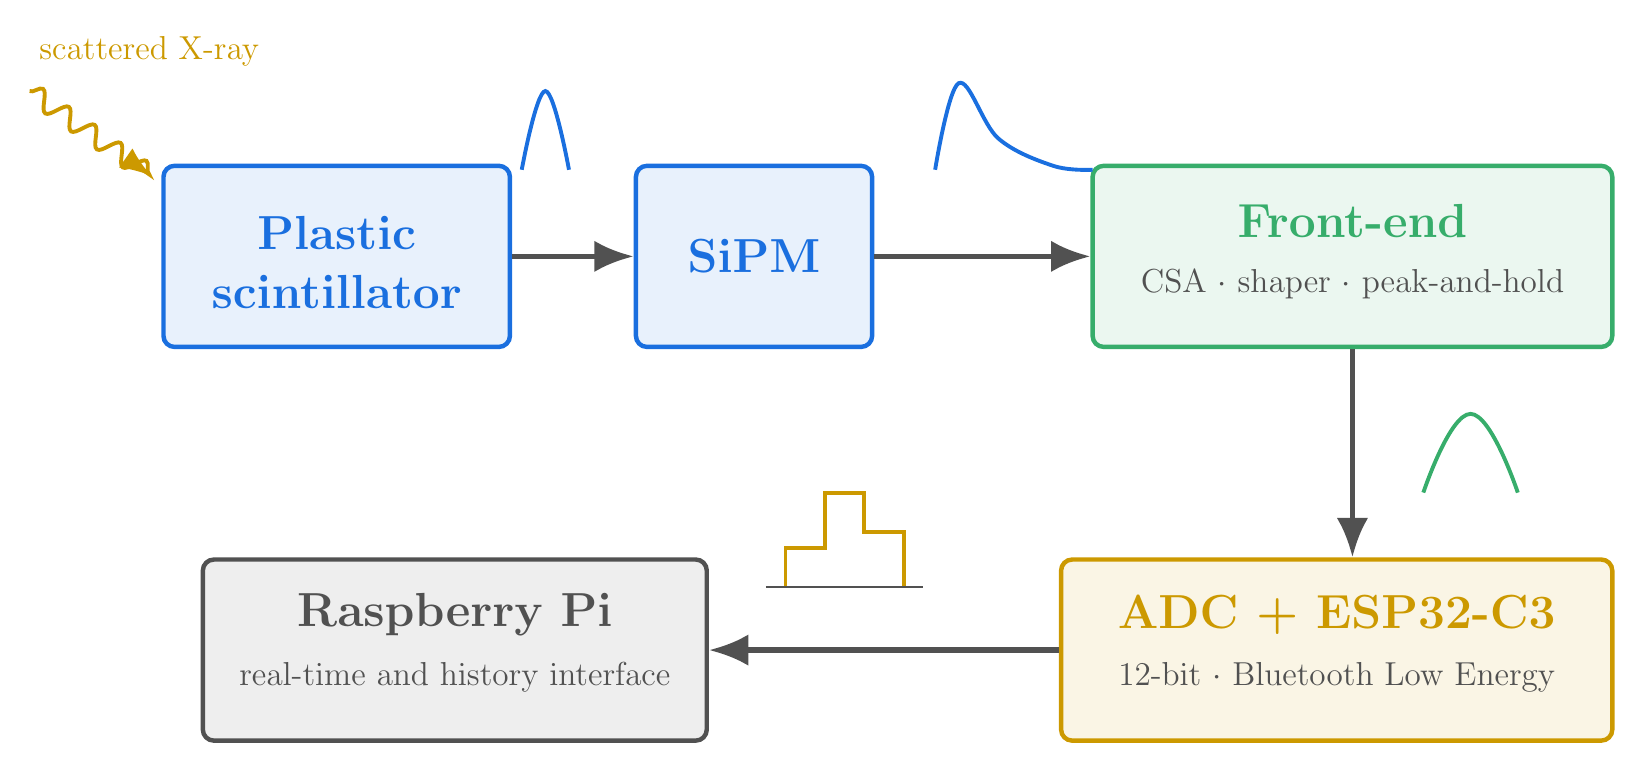
\begin{tikzpicture}[x=1cm, y=1cm,
  % ---- colours: your palette -----------------------------------------
  /utils/exec={%
    \definecolor{figblue}  {RGB}{ 26,111,223}%
    \definecolor{figgreen} {RGB}{ 55,173,107}%
    \definecolor{figyellow}{RGB}{204,153,  0}%
    \definecolor{figgrey}  {RGB}{ 81, 81, 81}%
  },
  % ---- one style per box, change fill/draw here ------------------------
  blk/.style={
    rounded corners=4pt, draw=#1, line width=1.6pt, fill=#1!10,
    align=center, inner sep=6pt, text=#1
  },
  ttl/.style={font=\LARGE\bfseries},
  sub/.style={font=\large, text=figgrey},
  flow/.style={draw=figgrey, line width=2pt, -{Latex[length=5mm,width=4mm]}},
  wave/.style={draw=#1, line width=1.4pt},
]

% =====================================================================
%  ROW 1 : detection and analogue front end
% =====================================================================
\node[blk=figblue,  minimum width=4.4cm, minimum height=2.3cm] (scint) at (2.7,6.4) {};
\node[ttl, text=figblue] at (2.7,6.7) {Plastic};
\node[ttl, text=figblue] at (2.7,5.95) {scintillator};

\node[blk=figblue,  minimum width=3.0cm, minimum height=2.3cm] (sipm)  at (8.0,6.4) {};
\node[ttl, text=figblue] at (8.0,6.4) {SiPM};

\node[blk=figgreen, minimum width=6.6cm, minimum height=2.3cm] (fe)    at (15.6,6.4) {};
\node[ttl, text=figgreen] at (15.6,6.85) {Front-end};
\node[sub]                at (15.6,6.05) {CSA $\cdot$ shaper $\cdot$ peak-and-hold};

% =====================================================================
%  ROW 2 : digitisation and readout
% =====================================================================
\node[blk=figyellow, minimum width=7.0cm, minimum height=2.3cm] (adc) at (15.4,1.4) {};
\node[ttl, text=figyellow] at (15.4,1.85) {ADC + ESP32-C3};
\node[sub]                 at (15.4,1.05) {12-bit $\cdot$ Bluetooth Low Energy};

\node[blk=figgrey, minimum width=6.4cm, minimum height=2.3cm] (rpi) at (4.2,1.4) {};
\node[ttl, text=figgrey] at (4.2,1.85) {Raspberry Pi};
\node[sub]               at (4.2,1.05) {real-time and history interface};

% =====================================================================
%  FLOW
% =====================================================================
\draw[flow] (scint) -- (sipm);
\draw[flow] (sipm)  -- (fe);
\draw[flow] (fe.south) -- (fe.south |- adc.north);
\draw[flow] (adc) -- (rpi);

% incoming scattered X-ray
\draw[wave=figyellow, decorate, decoration={snake, amplitude=1.2mm, segment length=4mm},
      -{Latex[length=4mm,width=3mm]}] (-1.2,8.5) -- (0.35,7.42);
\node[font=\large, text=figyellow, anchor=west] at (-1.2,9.0) {scattered X-ray};

% =====================================================================
%  WHAT THE SIGNAL LOOKS LIKE, one sketch per hand-off
% =====================================================================
% light flash out of the scintillator
\draw[wave=figblue] plot[smooth,tension=0.7] coordinates
      {(5.05,7.5) (5.35,8.5) (5.65,7.5)};
% raw SiPM pulse: fast rise, long tail
\draw[wave=figblue] plot[smooth,tension=0.6] coordinates
      {(10.3,7.5) (10.6,8.6) (11.1,7.9) (11.8,7.55) (12.3,7.5)};
% shaped pulse, beside the vertical arrow
\draw[wave=figgreen] plot[smooth,tension=0.8] coordinates
      {(16.5,3.4) (17.1,4.4) (17.7,3.4)};
% digitised spectrum, above the arrow back to the interface
\draw[wave=figyellow] (8.4,2.2) -- (8.4,2.7) -- (8.9,2.7) -- (8.9,3.4)
                   -- (9.4,3.4) -- (9.4,2.9) -- (9.9,2.9) -- (9.9,2.2);
\draw[figgrey, line width=1pt] (8.15,2.2) -- (10.15,2.2);

\end{tikzpicture}
